\documentclass[10pt]{article}

\usepackage[letterpaper,margin=1in]{geometry}
\usepackage[T1]{fontenc}
\usepackage{lmodern}
\usepackage{microtype}
\usepackage{amsmath,amssymb}
\usepackage{graphicx}
\usepackage{booktabs}
\usepackage{tabularx}
\usepackage{xcolor}
\usepackage{enumitem}
\usepackage{fvextra}
\usepackage{caption}
\usepackage{float}
\usepackage{needspace}
\usepackage{tikz}
\usetikzlibrary{arrows.meta,positioning,calc}
\usepackage[numbers,sort&compress]{natbib}
\usepackage[colorlinks=true,linkcolor=blue!50!black,citecolor=blue!50!black,urlcolor=blue!50!black]{hyperref}
\usepackage{url}

\captionsetup{font=small,labelfont=bf}
\setlist{itemsep=2pt,topsep=3pt}
\newcommand{\qsa}{QSA}
\newcommand{\code}[1]{\texttt{#1}}

\title{Quantum Sensing Agent: A Language-Model Agent for\\Operating NV-Center Quantum Sensing Experiments}

\author{
  Zechen Zhang$^{*}$ \quad Ruolan Xue$^{*}$ \quad Jack Fan \quad Amir Yacoby\\[4pt]
  Department of Physics, Harvard University, Cambridge, MA 02138, USA\\[2pt]
  {\small $^{*}$Equal contribution; Z.Z. and R.X. co-led this work. Correspondence: \href{mailto:zechen_zhang@g.harvard.edu}{\nolinkurl{zechen_zhang@g.harvard.edu}}, \href{mailto:ruolanxue@g.harvard.edu}{\nolinkurl{ruolanxue@g.harvard.edu}}}
}

\date{}

\begin{document}
\maketitle

\begin{abstract}
A quantum sensing experiment is a long chain of routine but judgment-laden steps: map the sample, pick an emitter, centre on it, focus, choose a microwave window, and decide whether a flat spectrum means a bad emitter or a bad setup.
We present the Quantum Sensing Agent (\qsa{}), a language-model agent that runs this chain on a room-temperature scanning-confocal setup for nitrogen-vacancy (NV) centers in diamond.
\qsa{} works through the laboratory's existing control software. It acts only by editing measurement configurations and launching allow-listed scripts, it reads the resulting plots with a vision model, and it plans the next measurement from what it sees.
Four design choices make this practical on real hardware: a configuration-level action space that keeps the instrument within its normal operating envelope, a collaboration model in which the scientist sets goals, adds domain knowledge and approves actions with adjustable autonomy, an experiential memory that stores past sessions together with their figures, and a model-agnostic engine layer.
Deployed in the Yacoby lab from February 2025, \qsa{} completed 73 measurements on the apparatus. In a representative session it worked through a list of candidate emitters, proposed diagnoses when two showed no resonance, and recorded an optically detected magnetic resonance spectrum on the third.
We describe the system, present case studies of the agent at work, and distill lessons for building agents for quantum laboratories. Code, session logs and data are open source.
\end{abstract}

% =====================================================================
\section{Introduction}
\label{sec:intro}

Experimental physics runs on a tight loop between measurement and judgment.
In a quantum sensing experiment with nitrogen-vacancy (NV) centers in diamond, a single characterization run already involves imaging the sample, deciding which bright spots are worth pursuing, centring and focusing on one of them, choosing a microwave frequency window and power, and interpreting the resulting optically detected magnetic resonance (ODMR) spectrum.
Classical automation speeds up individual steps, for example by choosing ODMR frequencies adaptively~\cite{dushenko2020odmr} or by focusing on point emitters without imaging~\cite{sahoo2023find}.
Deciding \emph{which} step to take next, and explaining in words why a measurement failed, has remained the experimenter's job.

Language-model agents that call tools are a natural candidate for this role.
When we began this project in early 2025, such agents had planned and executed chemistry experiments~\cite{boiko2023coscientist,bran2023chemcrow}, operated scanning-probe microscopes~\cite{liu2024microscopy,mandal2024aila}, and calibrated a superconducting quantum processor~\cite{cao2024kagents}; to our knowledge, none had yet operated a quantum-sensing experiment.
We set out to build one and to run it on a working NV setup, with the goal of learning what such an agent needs in order to be useful, safe and trustworthy at the bench.

This report describes the result, the Quantum Sensing Agent (\qsa{}; Figure~\ref{fig:arch}).
A scientist states a goal in plain language, such as ``characterize all the NVs in the field of view''.
\qsa{} then runs the measurement loop of a scanning-confocal microscope: confocal scan, emitter localization, focus optimization and an ODMR sweep, repeated for each candidate.
It configures each measurement, launches it through the lab's own scripts, inspects the plot, and decides what to do next, while the scientist can redirect it, add domain knowledge, or approve each action.

\needspace{6\baselineskip}
\paragraph{Contributions.}
\begin{enumerate}[leftmargin=*]
  \item \textbf{An agent harness for a quantum sensing apparatus} that sits on top of the lab's existing control software. Its configuration-level action space, which consists of reading and writing measurement configurations, running allow-listed scripts and reading plots, needs no new instrument drivers and confines the agent to what a careful user of the same scripts could do (Section~\ref{sec:system}).
  \item \textbf{A collaboration model with adjustable autonomy.} In assistant mode every consequential action needs the scientist's approval; in auto mode the agent proceeds on its own for a bounded number of steps. Throughout, the scientist can inject domain knowledge in natural language, which the agent turns into concrete measurement settings.
  \item \textbf{Experiential memory with figure provenance.} Past sessions are stored together with the plots they refer to, so the agent can recall earlier attempts and re-open their figures, a step towards agents that learn from their own experimental history.
  \item \textbf{A deployment on real hardware with case studies.} We report the agent's work on an NV setup from February to June 2025, including end-to-end emitter characterization, in-session adoption of expert rules, diagnosis of failed measurements, and an instructive failure mode under autonomy (Sections~\ref{sec:deployment} and~\ref{sec:cases}). We distill these into design lessons and release the code, logs and data.
\end{enumerate}
The engine layer is model-agnostic: the deployment used Claude, and the same harness runs with other model families through an OpenAI-compatible adapter (Section~\ref{sec:engine}).

% =====================================================================
\section{Background and related work}
\label{sec:related}

\paragraph{NV centers and ODMR.}
The negatively charged NV center has a spin-1 ground state whose $m_s=\pm1$ levels lie $D\approx2.87$\,GHz above $m_s=0$ at room temperature~\cite{doherty2013nv}.
A magnetic field component $B_\parallel$ along the NV axis splits the $\pm1$ levels by $2\gamma B_\parallel$, with $\gamma\approx2.8$\,MHz/G.
Green excitation polarizes the spin into $m_s=0$, and the $\pm1$ states fluoresce less, so a resonant microwave field appears as a dip in the photon count rate.
Sweeping the microwave frequency yields the ODMR spectrum, the basic readout for NV magnetometry and the measurement \qsa{} targets.

\paragraph{Language-model agents in the laboratory.}
Coscientist~\cite{boiko2023coscientist} and ChemCrow~\cite{bran2023chemcrow} established the pattern of a language model combined with tools and instrument interfaces in chemistry; self-driving laboratories more broadly are reviewed in~\cite{tom2024sdl}.
In microscopy, language models have operated scanning-probe instruments~\cite{liu2024microscopy}, and the AILA benchmark found that frontier models can be fragile and deviate from instructions when operating an atomic force microscope~\cite{mandal2024aila}, a finding that motivates the restrictive action space of \qsa{}.
Later agents run X-ray beamlines with human corrections stored as memory~\cite{vriza2025learnonjob}, multistage accelerator experiments~\cite{hellert2025accelerator} and cryogenic transport measurements~\cite{bauer2026transport}.

\paragraph{Agents for quantum hardware.}
k-agents~\cite{cao2024kagents} calibrated a superconducting quantum processor with language-model agents, and subsequent work has addressed superconducting qubits~\cite{li2026scqubit,xu2026vibe,fan2026qmclaw}, trapped ions with hardware-safety gates~\cite{wang2026artiq}, neutral atoms~\cite{dalyac2026neutralatom} and optics~\cite{uddin2025optics,lopez2026opticsvlm}.
For quantum sensing, QCopilot~\cite{sha2025qcopilot} optimizes laser cooling for a cold-atom sensor with a knowledge base of past experiments, and Isogawa et al.~\cite{isogawa2026nv} operate a confocal NV setup and run pulsed protocols autonomously over many hours.
Both appeared after \qsa{} was deployed; we discuss how they extend the approach in Section~\ref{sec:discussion}.
Classical automation of NV experiments, such as adaptive Bayesian measurement design~\cite{bonato2015adaptive,santagati2018magnetic,dushenko2020odmr,mcmichael2021ramsey}, optimizes \emph{within} a fixed protocol; an agent decides \emph{which} protocol to run next, and the two are complementary.

\paragraph{Agent memory.}
Retrieval-augmented generation~\cite{lewis2020rag} and episodic or reflective memories~\cite{shinn2023reflexion,park2023generative,wang2023voyager,zhao2023expel} let agents reuse past experience, and trajectory retrieval is a strong foundation for agent memory, especially when combined with fine-tuning~\cite{ferraz2026exprag}.
\qsa{} applies this idea to a laboratory, and stores with each memory the figures it refers to, so that the agent can look at the evidence again rather than rely on a text summary.

% =====================================================================
\section{The \qsa{} harness}
\label{sec:system}

\begin{figure}[t]
  \centering
  \resizebox{\linewidth}{!}{% Figure 1: architecture of the Quantum Sensing Agent harness
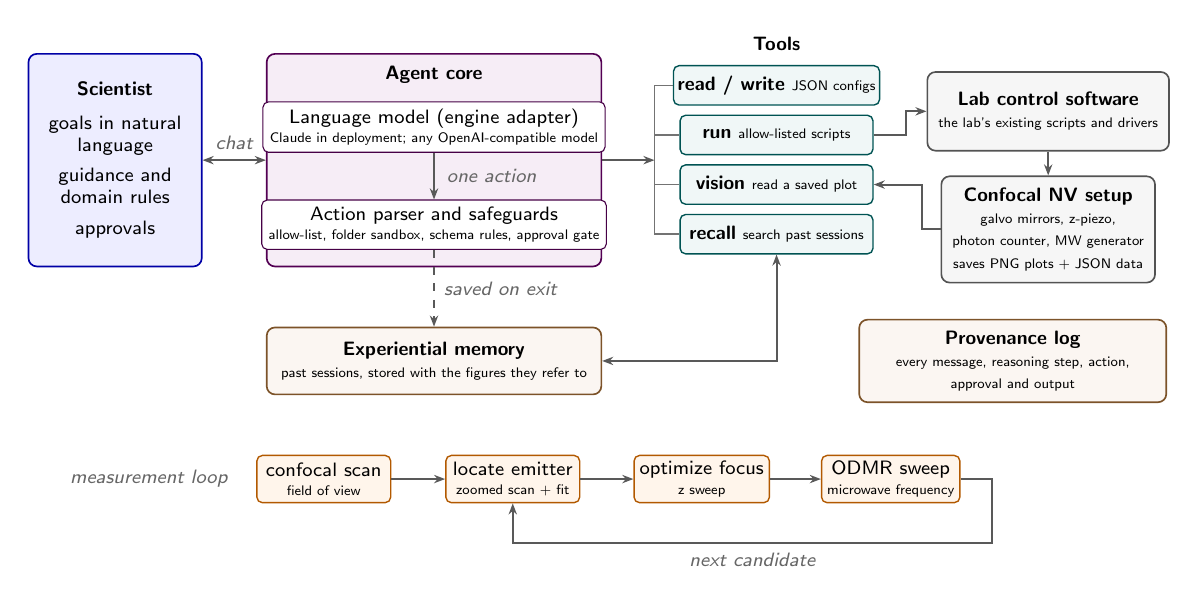
\begin{tikzpicture}[
  font=\sffamily\scriptsize,
  >={Stealth[length=4pt]},
  box/.style={draw=#1!65!black, fill=#1!7, rounded corners=3pt, line width=0.6pt, align=center, inner sep=4pt},
  inner/.style={draw=violet!55!black, fill=white, rounded corners=2pt, align=center, minimum width=3.85cm, inner sep=2.5pt},
  tool/.style={draw=teal!65!black, fill=teal!6, rounded corners=2pt, line width=0.5pt, align=center,
               minimum width=2.45cm, minimum height=0.5cm, inner sep=1.5pt},
  wstep/.style={draw=orange!70!black, fill=orange!8, rounded corners=2pt, line width=0.5pt, align=center,
               minimum width=1.7cm, minimum height=0.6cm, inner sep=2pt},
  lab/.style={font=\sffamily\scriptsize\itshape, text=black!60},
  flow/.style={->, line width=0.7pt, draw=black!65},
]

% ---------------- scientist
\node[box=blue, minimum width=2.2cm, minimum height=2.7cm] (sci) at (0,0)
  {\textbf{Scientist}\\[4pt] goals in natural\\language\\[3pt] guidance and\\domain rules\\[3pt] approvals};

% ---------------- agent core
\node[box=violet, minimum width=4.25cm, minimum height=2.7cm] (core) at (4.05,0) {};
\node[font=\sffamily\scriptsize\bfseries, anchor=north] at ([yshift=-1pt]core.north) {Agent core};
\node[inner] (llm) at (4.05,0.42) {Language model (engine adapter)\\[-1pt] {\tiny Claude in deployment; any OpenAI-compatible model}};
\node[inner] (guard) at (4.05,-0.82) {Action parser and safeguards\\[-1pt] {\tiny allow-list, folder sandbox, schema rules, approval gate}};
\draw[flow] (llm.south) -- node[right, lab, xshift=1pt] {one action} (guard.north);

% ---------------- tools
\node[font=\sffamily\scriptsize\bfseries] at (8.4,1.48) {Tools};
\node[tool] (tcfg) at (8.4, 0.95) {\textbf{read / write}\ {\tiny JSON configs}};
\node[tool] (trun) at (8.4, 0.32) {\textbf{run}\ {\tiny allow-listed scripts}};
\node[tool] (tvis) at (8.4,-0.31) {\textbf{vision}\ {\tiny read a saved plot}};
\node[tool] (tmem) at (8.4,-0.94) {\textbf{recall}\ {\tiny search past sessions}};
\draw[line width=0.6pt, draw=black!55] (6.85,0.95) -- (6.85,-0.94);
\foreach \t in {tcfg,trun,tvis,tmem}{ \draw[line width=0.6pt, draw=black!55] (6.85,0 |- \t.west) -- (\t.west); }
\draw[flow] (core.east) -- (6.85,0);

% ---------------- lab
\node[box=gray, minimum width=2.55cm, minimum height=1.0cm] (stack) at (11.85,0.62)
  {\textbf{Lab control software}\\{\tiny the lab's existing scripts and drivers}};
\node[box=gray, minimum width=2.55cm, minimum height=1.35cm] (hw) at (11.85,-0.88)
  {\textbf{Confocal NV setup}\\{\tiny galvo mirrors, z-piezo,}\\{\tiny photon counter, MW generator}\\{\tiny saves PNG plots + JSON data}};
\draw[flow] (trun.east) -- (10.05,0.32) |- (stack.west);
\draw[flow] (stack) -- (hw);
\draw[flow] (hw.west) -- (10.25,-0.88) |- (tvis.east);

% ---------------- memory & log
\node[box=brown, minimum width=4.25cm, minimum height=0.85cm] (mem) at (4.05,-2.55)
  {\textbf{Experiential memory}\\{\tiny past sessions, stored with the figures they refer to}};
\node[box=brown, minimum width=3.9cm, minimum height=0.85cm] (log) at (11.4,-2.55)
  {\textbf{Provenance log}\\{\tiny every message, reasoning step, action,}\\{\tiny approval and output}};
\draw[flow, <->] (tmem.south) |- (mem.east);
\draw[flow, dashed] (guard.south) -- node[right, lab] {saved on exit} (mem.north);

% ---------------- the scientist loop
\draw[flow, <->] (sci.east) -- node[above, lab] {chat} (core.west);

% ---------------- workflow strip
\node[lab, anchor=east] at (1.55,-4.05) {measurement loop};
\node[wstep] (s1) at (2.65,-4.05) {confocal scan\\[-1pt]{\tiny field of view}};
\node[wstep] (s2) at (5.05,-4.05) {locate emitter\\[-1pt]{\tiny zoomed scan + fit}};
\node[wstep] (s3) at (7.45,-4.05) {optimize focus\\[-1pt]{\tiny z sweep}};
\node[wstep] (s4) at (9.85,-4.05) {ODMR sweep\\[-1pt]{\tiny microwave frequency}};
\draw[flow] (s1) -- (s2); \draw[flow] (s2) -- (s3); \draw[flow] (s3) -- (s4);
\draw[flow] (s4.east) -- ++(0.4,0) |- ([yshift=-0.5cm]s2.south) node[pos=0.75, below, lab] {next candidate} -- (s2.south);
\end{tikzpicture}
}
  \caption{Architecture of \qsa{}. The scientist states goals, adds domain knowledge and approves actions in a chat. In each turn the language model reasons and proposes one action, which passes through the action parser and its safeguards before reaching a tool. Measurements are launched through the lab's existing control software, and the saved plots come back to the agent through the vision tool. Sessions are stored in an experiential memory together with the figures they refer to, and every step is recorded in a provenance log. Bottom: the measurement loop the agent runs for each candidate emitter.}
  \label{fig:arch}
\end{figure}

\subsection{Design goals}
We designed \qsa{} around five requirements that come from working at a real optical bench rather than in simulation:
\begin{enumerate}[leftmargin=*]
  \item \textbf{Use what the lab already has.} The agent must work through the existing, trusted control software and measurement scripts, so that adopting it requires no new instrument drivers.
  \item \textbf{Bounded actions.} The agent should only be able to do what a careful user of those scripts could do, and every action should be inspectable before it runs.
  \item \textbf{Decide from the same evidence as a physicist.} The agent should read the plots an experimenter reads, and plan the next measurement from them.
  \item \textbf{Keep the scientist in charge.} Domain knowledge and approvals should flow naturally from the scientist to the agent, with autonomy that can be dialled up as trust grows.
  \item \textbf{Accumulate experience and leave a record.} The agent should be able to recall earlier sessions, and every measurement should be traceable to the reasoning and configuration that produced it.
\end{enumerate}

\subsection{Agent loop}
\label{sec:loop}
Each turn of the loop is one language-model call.
The prompt consists of a system instruction, which states the overall goal, the measurement workflow, each script's inputs, outputs and caveats, and the rules below (abridged in Appendix~\ref{app:prompt}), followed by the conversation so far.
The model answers with a \code{<think>} block, in which it reasons about the current state, and an \code{<action>} block containing a JSON object.
The harness parses the action, applies the safeguards, executes it, and appends the result (script output, a file's content, or the vision model's reading of a plot) to the conversation, so that the next turn sees it.
The loop returns control to the scientist whenever the agent sends a message.

\subsection{A configuration-level action space}
\label{sec:actions}
The agent acts through six action types: \code{message} (talk to the scientist), \code{read} and \code{write} (a measurement configuration), \code{run} (launch a measurement script), \code{vision} (read a saved plot) and \code{recall} (search past sessions; \code{rag\_search} in the code).
Measurements are four thin wrappers around the lab's control software: \code{galvo\_scan} (a confocal raster of the field of view), \code{find\_nv} (a zoomed scan with a 2D Gaussian fit that moves the beam onto the emitter), \code{optimize} (a focus sweep) and \code{ESR} (a continuous-wave ODMR sweep).
Each wrapper loads a JSON configuration, runs the corresponding toolkit routine, and saves a plot and a data file.

This interface is the central design choice.
The agent never touches instrument drivers.
It changes a measurement only by writing a new configuration, and the system instruction requires it to start from the default configuration and change parameter values only, never keys, structure or types (Appendix~\ref{app:config}).
The \code{run} command must match a fixed pattern and name one of the four allow-listed scripts, and reads and writes are confined to the run's configuration and data folders.
As a result, the agent's reach is exactly the envelope of the lab's own scripts with their own parameter ranges: anything it can do, a careful student could do with the same scripts.
The same interface makes the harness portable, since adapting it to another setup means wrapping that setup's scripts and describing them in the system instruction.

\subsection{Perception through plots}
After each measurement the agent can send the saved plot, together with recent conversational context, to a vision-capable model and receive a description: where the bright spots are in a confocal image, whether the zoomed scan is centred, where the focus curve peaks, and whether an ODMR spectrum shows a dip.
Reading the same figures as the experimenter keeps the agent's decisions grounded in evidence a human can check, and lets the scientist correct its reading when needed.

\subsection{Collaboration and adjustable autonomy}
\label{sec:modes}
\qsa{} is built for collaboration rather than replacement.
In \emph{assistant mode}, every \code{write}, \code{run} and \code{vision} action waits for an explicit ``yes'' from the scientist at the console, and a refusal is fed back to the agent so that it can revise its plan.
In \emph{auto mode}, permissions are granted and logged automatically, and the agent continues until it addresses the scientist or reaches a cap of ten consecutive steps.
The harness executes only the first action of each reply, so that every step is observed before the next is planned.

Throughout a session the scientist can steer the agent in natural language, at any level of detail: a coordinate list read off a scan, a frequency window to try, or a general rule of thumb (``an ODMR count rate far below the \code{find\_nv} rate suggests a quenched NV''). In practice the scientists tagged such rules (\code{\#rule}, \code{\#experience}, \code{\#suggest}) to flag them as reusable knowledge.
The agent's role is to turn this guidance into correct measurement settings and to carry the bookkeeping of a long session: which candidates have been tried, which settings were used, and what came out.

\subsection{Experiential memory}
\label{sec:memory}
A lab agent should learn from earlier attempts: which windows showed resonances, which candidates were dead, which parameters failed.
When a session ends, \qsa{} splits the conversation into overlapping chunks of ten turns, embeds each chunk with a sentence-transformer model~\cite{wang2020minilm}, and stores it together with the names of the plots it mentions.
When the agent is stuck or wants precedent, it issues a \code{recall} action; the most similar chunks are inserted into the prompt in a clearly delimited block, and the agent can re-open the historical plots they reference through the \code{vision} action.
Storing figure provenance alongside text means that the agent revisits the evidence itself, not only an earlier model's description of it.
An earlier version retrieved context automatically on every turn; making recall an explicit action lets the agent decide when history is relevant.

\subsection{A model-agnostic engine layer}
\label{sec:engine}
The harness talks to language models through two functions only: one for text reasoning and one for reading a plot.
Changing the model means changing this adapter, selected by an environment variable; the prompt, tools, safeguards and memory are unchanged.
The deployment used Claude through the Anthropic API (Claude 3.5 Sonnet in February 2025 and Claude 3.7 Sonnet, including plot reading, from March onward).
The release adds an adapter for any OpenAI-compatible endpoint, which covers hosted models from other providers and locally served open models.
As a check, we ran the unchanged harness with GPT-6 through this adapter. Given the same opening request as in our deployment, it produced well-formed reasoning and a single action: a message asking permission to begin with a confocal scan of the field of view, as the assistant-mode instruction requires. Current models also read our recorded plots well (Section~\ref{sec:discussion}).

\subsection{Provenance}
Every session creates a run folder with the configurations the agent wrote, the data and plots the scripts saved, and a time-stamped log of every message, reasoning block, action, approval and script output.
Any measurement can therefore be traced back to the request, reasoning and configuration that produced it.
This record made the case studies below possible, and it is what allowed us to spot and understand the failure mode described in Section~\ref{sec:case-fail}.

% =====================================================================
\section{Deployment}
\label{sec:deployment}

\paragraph{Apparatus.}
The setup is a room-temperature scanning-confocal microscope for NV centers in diamond, controlled from a Windows PC by the lab's Python control stack (\code{pylabcontrol} with \code{b26\_toolkit}).
A data-acquisition card steers the galvanometer mirrors and the objective's z-piezo and counts photons; a Rohde~\&~Schwarz signal generator supplies the microwaves.
Samples included a diamond with a pillar array of NVs and fields of individual NVs.
Further details are in Appendix~\ref{app:apparatus}.

\paragraph{Record.}
\qsa{} ran its first session on the apparatus on 18 February 2025.
From then to June 2025 it completed 73 measurements in 16 sessions on 10 days (Figure~\ref{fig:deploy}): 20 confocal scans, 27 emitter localizations, 8 focus optimizations and 18 ODMR sweeps.
Most instrument time went into ODMR, with a median sweep of 14 minutes, while scans, localizations and focus sweeps each took under a minute.
The agent's own overhead was small by comparison: the median language-model call took 8\,s, and the scientist's median reply 16\,s.
The richest sessions, on 19 April and 14 May, each ran for more than three hours.

\begin{figure}[t]
  \centering
  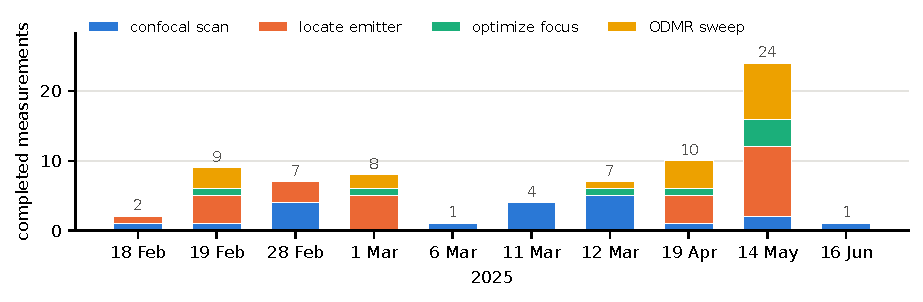
\includegraphics[width=0.84\linewidth]{figures/fig_deployment.pdf}
  \caption{Measurements completed by \qsa{} on the NV setup, per day of operation and by type. The first session on the apparatus was on 18 February 2025; 14 May is the case study of Section~\ref{sec:case-chain}.}
  \label{fig:deploy}
\end{figure}

The deployment was a collaboration between the agent and two experimenters at the setup, who supervised every session; in most sessions each consequential action required their approval.
Over these months the harness evolved from a first prototype (February--March) through a refactored lab version (April) and a version with memory of past sessions (May) to a release with explicit assistant and auto modes and one action per turn (June).

% =====================================================================
\section{Case studies}
\label{sec:cases}

\subsection{End-to-end characterization of NV candidates}
\label{sec:case-chain}

\begin{figure}[t]
  \centering
  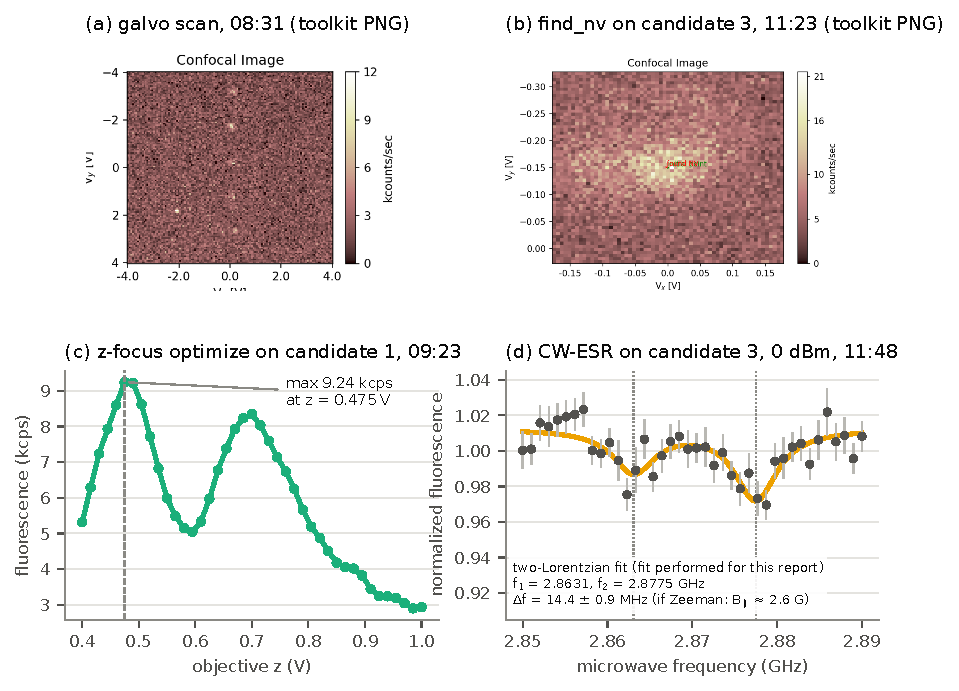
\includegraphics[width=0.86\linewidth]{figures/fig2_case_chain_14may.pdf}
  \caption{One session of \qsa{} on 14 May 2025. (a) Confocal scan of the field of view, from which six candidate emitters were selected. (b) Zoomed scan on candidate 3 after centring. (c) Focus optimization on candidate 1. (d) ODMR sweep on candidate 3 (2.85--2.89\,GHz, 40 points, 0\,dBm, 50 averages), with a two-Lorentzian fit performed for this report. Panels (a) and (b) are the lab software's own plots, as saved during the session.}
  \label{fig:case}
\end{figure}

On 14 May 2025 the scientist opened a session with the request ``characterize all the NV in the field of view''.
The agent read the default scan configuration, wrote its own, and ran a confocal scan of the field of view (Figure~\ref{fig:case}a).
The scientist read six candidate positions off the image and asked the agent to remember them; the agent then worked through the list over the next 3.4 hours.
For each candidate it wrote a localization configuration centred on the given coordinates, optimized the focus where needed (Figure~\ref{fig:case}c), and ran ODMR sweeps over windows and powers chosen together with the scientist.
The first two candidates showed no clear resonance (Section~\ref{sec:case-diag}).
On the third, the scientist asked for a 2.85--2.89\,GHz window at 0\,dBm; the agent wrote exactly these settings, and the sweep showed two clear dips (Figure~\ref{fig:case}d), at which point the scientist noted ``good we see ESR'' and the agent moved on to the next candidate.

A two-Lorentzian fit to this spectrum, which we performed for this report, is strongly preferred over a single dip.
The dips sit at $2863.1\pm0.8$ and $2877.5\pm0.5$\,MHz with contrasts of 2--4\%, symmetric about $D$, with a splitting of $14.4\pm0.9$\,MHz.
Read as a Zeeman splitting this would correspond to $B_\parallel\approx2.6$\,G, but the bias field during the session was not recorded and strain can also split the resonance, so we do not attribute it to a specific field.
The point of the case is the chain itself: from a single sentence, the agent carried six candidates through imaging, localization, focusing and ODMR, keeping the bookkeeping of a multi-hour session while the scientist made the scientific calls.

\subsection{Turning expert knowledge into measurements}
\label{sec:case-guidance}
In a session on 19 April 2025 the scientist taught the agent rules of thumb as it worked.
One message, tagged \code{\#experience}, noted that single-NV ODMR contrast ranges from ``a few percent (bad) to 20\% (best)'' and suggested scanning 2.80--2.84\,GHz; the agent restated the point in its reasoning and wrote a configuration for that window.
Another, tagged \code{\#suggest}, observed that a count rate during ODMR far below the localization count rate suggests the NV has been quenched, in which case one should move on.
The agent immediately applied the rule to its current candidate: it compared the localization rate of 11.5\,kcps with the 2.9\,kcps seen during the sweep, concluded that the emitter had quenched, abandoned it, and moved to the next candidate on its list.
Across the deployment, every instruction that specified coordinates, a frequency window or a power (22 in total) appeared exactly in the next configuration the agent wrote.
This kind of fidelity is what lets the scientist delegate the mechanics of a measurement while keeping control of its content.

\subsection{Diagnosing a missing resonance}
\label{sec:case-diag}
Returning to 14 May: after five sweeps on the first two candidates showed no clear dip, the scientist asked ``can you look at the historical attempts and tell me why we are not seeing ESR for many attempts?''.
The agent reviewed the session and organized its answer into three groups of hypotheses:
\begin{itemize}[leftmargin=*]
  \item \emph{Microwave delivery}: the antenna or wire position, or the power reaching the NV.
  \item \emph{Properties of the NVs}: misalignment with the field, a different charge state, or resonances outside the swept window.
  \item \emph{Equipment status}: recurring status messages from the pulse generator in the measurement output.
\end{itemize}
The scientist checked the microwave delivery physically, found it working, and moved on to the third candidate, which showed the resonance of Figure~\ref{fig:case}d.
The agent could not run the decisive test itself, but its structured diagnosis gave the experimenter a checklist and kept the session moving.

\subsection{Recovering from a tool error}
\label{sec:case-recover}
Later the same day the agent passed a configuration key (\code{esr\_RnS}) where the run command expected a script name.
The command parser rejected it and returned an error; on its next turn the agent identified the mistake (``correct the script path to use \code{ESR} instead of \code{esr\_RnS}''), re-issued the command, and the sweep completed.
The fixed command format turned a potential silent failure into an explicit error the agent could act on.

\subsection{A cautionary case: autonomy without grounding}
\label{sec:case-fail}
On 16 June 2025 we tried the new auto mode on the apparatus with a single instruction, ``characterize NV for me''.
The agent ran a confocal scan and read the plot, which worked as intended.
In its next replies, however, the model continued the conversation on its own and wrote text that looked like the output of a localization, a focus optimization and an ODMR sweep, including ``ESR transitions found at 2.8671 GHz, 2.8732 GHz''.
None of these measurements had run: the one-action-per-turn rule stopped the invented actions from executing, and the real commands that followed failed because the configurations they referred to did not exist.
The agent nevertheless treated the invented results as real, carried them into a recall query, and reported them in its summary.

This failure has a clear mechanism.
The harness serialized the whole history into a single text transcript of \code{User:} and \code{Assistant:} turns, and a language model will sometimes continue such a transcript, writing the other side's lines and the tool's output.
In assistant mode this was caught at the approval step, and the scientist refused actions that came from such replies.
In auto mode nobody was in the loop to notice.
The lesson, which we develop below, is that tool output must be marked by the harness in a way the model cannot imitate, and that autonomy should be granted only together with such grounding.

% =====================================================================
\section{Discussion}
\label{sec:discussion}

\paragraph{What worked.}
A general-purpose language model, without any hardware-specific training, operated the measurement chain of a real NV setup through a narrow, text-based interface.
It translated the scientist's instructions into exactly the requested settings, kept a multi-candidate plan across hours, recovered from errors when the harness reported them explicitly, and offered useful hypotheses when a measurement failed.
Because it acted only through the lab's own scripts and their configurations, its mistakes stayed within what an ordinary user of those scripts could do, and the provenance log made every step auditable after the fact.

\paragraph{What was hard.}
The scientifically decisive judgments stayed with the experimenters: which spots were NVs, where to centre, which window to try, when an emitter had quenched, and whether the microwaves reached the sample.
In 2025, reading coordinates off a confocal image was unreliable, and the scientist usually supplied or corrected them.
This has changed quickly.
Re-reading the recorded 14 May scan with the harness's vision call in October 2026, Claude Opus 5.5 identified the same six spots the scientist had picked by eye, and GPT-6 identified four of them, without any change to the harness.
ODMR contrast in the deployment was low, and \qsa{} ran only continuous-wave protocols; pulsed sequences, where automation helps most, were out of scope.
Finally, the experiential memory was built and exercised during development, but the deployment was too short to evaluate whether recalling past sessions improves the agent's decisions; that evaluation is future work.

\paragraph{Lessons for agents in quantum laboratories.}
\begin{enumerate}[leftmargin=*]
  \item \emph{Keep the action space at the configuration level.} Wrapping the lab's own scripts gave a safe, portable interface; the agent never needed driver access.
  \item \emph{Separate tool output from model output.} Use structured messages for tool results, never a flat transcript, so that the model cannot write the instrument's side of the conversation.
  \item \emph{Grant autonomy together with grounding.} Approval gates did real work. Before removing them, the harness should verify that every result the agent reasons about was produced by an instrument.
  \item \emph{Give the agent numerical tools for numerical questions.} Peak finding, fitting and spot detection belong in tools, and the model's role is to decide when to use them.
  \item \emph{Make expert knowledge persistent and explicit.} The scientist's tagged rules of thumb were exactly the knowledge that should carry across sessions; a small curated store of lab rules would complement retrieval over raw conversations.
\end{enumerate}

\paragraph{Since early 2025.}
The field has moved quickly.
Subsequent systems have formalized per-action authorization~\cite{wang2026artiq}, kept persistent laboratory memories~\cite{sha2025qcopilot,vriza2025learnonjob}, separated rule engines from language-model reasoning~\cite{fan2026qmclaw}, and, on NV centers, run pulsed protocols autonomously over many hours~\cite{isogawa2026nv}.
\qsa{} was an early point on this trajectory, with a human closely in the loop, and we hope that its design and the record of what it could and could not do are useful to others building such agents.

\section{Conclusion}
We built the Quantum Sensing Agent to find out whether a language model could run a quantum sensing experiment on a real apparatus, and deployed it on an NV-center confocal setup from February 2025.
By acting through the lab's existing scripts, reading the same plots as the experimenter, keeping the scientist in charge with adjustable autonomy, and recording every step, it carried out complete characterization chains on real NV centers.
Its failures were as informative as its successes, and point to the ingredients that agents for quantum laboratories need: grounded tool interfaces, explicit expert knowledge, and autonomy that grows with verification.

% =====================================================================
\section*{Code and data availability}
The code, configurations, session logs and the 14 May 2025 measurement data are available at \url{https://github.com/zechenzhangAGI/quantum-sensing-agent} under the MIT License, together with the scripts that reproduce the figures in this report.

\section*{Author contributions}
Z.Z. and R.X. co-led the project and performed the experiments together.
Z.Z. designed and built the agent harness: its architecture, action interface, collaboration modes and experiential memory.
R.X. proposed the experimental workflow and led the hardware side: the confocal NV setup and the measurement scripts through which the agent drives it.
J.F. contributed to the early agent code and the first memory prototype.
A.Y. supervised the work and provided the experimental platform.

\section*{Acknowledgments}
We thank the members of the Yacoby lab and the other contributors to the open-source repository.
AI assistants were used to help analyze session logs and prepare this manuscript; the authors take full responsibility for its content.

\bibliographystyle{plainnat}
\bibliography{refs}

% =====================================================================
\clearpage
\appendix
\sloppy

\section{Apparatus and measurement scripts}
\label{app:apparatus}
An NI~6353 data-acquisition card steers the galvo mirrors and the z-piezo with analog outputs and counts photons with a counter input; a Rohde~\&~Schwarz generator, addressed over VISA, provides the microwaves; a SpinCore PulseBlaster is initialized by every script. Positions are given as control voltages.
\code{galvo\_scan} rasters the field of view (default $126\times126$ points over $\pm4$\,V, 2\,ms per point); bright spots are NV candidates.
\code{find\_nv} takes a $61\times61$ zoomed scan over a 0.35\,V square around a chosen point, fits a 2D Gaussian and moves the beam to the fitted maximum.
\code{optimize} maximizes the count rate with 1D sweeps (by default 41 points in z over 0.6\,V).
\code{ESR} sweeps the microwave frequency between \code{freq\_start} and \code{freq\_stop} at power \code{power\_out}, averaging \code{esr\_avg} times and normalizing to a reference (default 2.90--2.95\,GHz, 100 points, $-8$\,dBm).

\section{Abridged system instruction}
\label{app:prompt}
The assistant-mode system instruction of the June 2025 version, abridged; ``[...]'' marks omissions.

\begin{Verbatim}[fontsize=\footnotesize,breaklines=true,breakanywhere=true,frame=single,framesep=2mm]
You are the NVExperimentAgent operating in ASSISTANT MODE, a specialized
assistant for nitrogen-vacancy (NV) center experiments in diamond chips.

OVERALL GOAL: Your primary objective is to utilize the available experimental
scripts to systematically measure the ESR (Electron Spin Resonance) of multiple
NV centers in a diamond chip. [...]

ASSISTANT MODE BEHAVIOR: [...] You must ask for permission before taking any
actions that modify files or run experiments. [...]

AVAILABLE EXPERIMENTAL SCRIPTS:
1. galvo_scan: Performs a coarse scan of the entire diamond chip [...]
   - ANALYSIS: Bright spots indicate potential NV centers, but results should
     be verified with find_nv
2. find_nv: [...] High-resolution brightness map with 2D Gaussian fit results
3. optimize: Performs 1D scans in X, Y, and Z directions [...]
4. ESR: [...] Fitted Gaussian minima (red labels) indicate ESR resonance
   frequencies, typically around 2.87 GHz for NV centers

TYPICAL WORKFLOW:
- Start with galvo_scan to map the chip and identify NV locations
- Use find_nv to precisely locate individual NVs from the coarse scan
- Run optimize to achieve optimal focus for measurements
- Perform ESR measurements on the located and optimized NV centers
[...]
2) Actions:
   - IMPORTANT: You may produce exactly ONE <action> block per response
   - The "type" must be one of: "message", "read", "write", "run", "vision",
     or "rag_search".
3) Security & Directory Rules:
   - Read Access: Only from the configs\ or data\ directories.
   - Write Access: Only to the configs\ or data\ directories.
   - Run Access: Only scripts in the scripts\ directory.
[...]
7) Configuration Management & Usage Flow:
   - CRITICAL: When writing new configs, you MUST maintain the EXACT same
     structure and format as the default config
   - CRITICAL: Only modify parameter values, never change keys, structure,
     or data types
   - Always read the appropriate default config first [...]
8) Behavior & Permissions:
   - When you <write> a file, ask the user permission. If denied, do not write.
   - When you <run> or <vision> a command, ask the user permission. [...]
11) RAG Search Tool:
   - When you feel stuck, need to learn from past experience, or believe
     relevant information exists in previous conversations, use the
     "rag_search" tool [...]
   - Historical Plot Analysis: When RAG search returns references to
     historical plots [...], you can analyze those plots using vision action
     with the full historical path
\end{Verbatim}

\section{Configuration example}
\label{app:config}
The default ODMR configuration; the agent may change values under \code{settings} only. The instrument address and lab-PC path are redacted.
\begin{Verbatim}[fontsize=\footnotesize,frame=single,framesep=2mm]
{ "scripts": { "esr_RnS": {
    "class": "ESR",
    "filepath": "<lab PC path>\\b26_toolkit\\scripts\\esr_RnS.py",
    "info": "ESR measurement script using R&S microwave generator",
    "instruments": {
      "microwave_generator": { "class": "R8SMicrowaveGenerator",
                               "settings": { "VISA_address": "<redacted>" } },
      "NI6353": { "class": "NI6353", "settings": {} },
      "PB":     { "class": "LISE607RTPulseBlaster", "settings": {} } },
    "settings": {
      "power_out": -8.0, "esr_avg": 100,
      "freq_start": 2.9e9, "freq_stop": 2.95e9, "range_type": "start_stop",
      "freq_points": 100, "integration_time": 0.05, "num_samps_per_pt": 100,
      "mw_generator_switching_time": 0.01, "turn_off_after": true,
      "norm_to_ref": true, "save_full_esr": true, "daq_type": "PCI",
      "fit_constants": { "num_of_peaks": -1, "minimum_counts": 0.9,
                         "contrast_factor": 3.0,
                         "zfs": 2.87e9, "gama": 2.8028e6 },
      "track_laser_power": { "on/off": false, "ai_channel": "ai4" } } } } }
\end{Verbatim}
For the candidate-3 sweep on 14 May the agent changed exactly five values: \code{freq\_start}\,=\,2.85e9, \code{freq\_stop}\,=\,2.89e9, \code{freq\_points}\,=\,40, \code{esr\_avg}\,=\,50 and \code{power\_out}\,=\,0.0.

\section{Excerpts from the 14 May session}
\label{app:excerpts}
Scientist messages and the agent's diagnosis, quoted from the session log (abridged).
\begin{Verbatim}[fontsize=\scriptsize,breaklines=true,breakanywhere=true,frame=single,framesep=2mm]
[08:29] USER: characterize all the NV in the field of view
[09:01] USER: i read the spot as (0.2,-3.3),(0.2,-1.8),(0.2,-0.3),(0.2,1.4),(0.2,2.8),(2,1.9)
[09:02] USER: remember the locations, you need to run find NV on the first NV
[10:03] USER: we may see or didn't see ESR, could be this NV having problem or the MW delivery
        has problem. Let us move to the next NV on our list
[10:57] USER: can you look at the historical attempts and tell me why we are not seeing ESR
        for many attempts?
        AGENT: 1. Microwave delivery: might have a problem with the MW antenna/wire position
           or connection [...] 2. NV properties: the NVs might be misaligned with our
           magnetic field; could be in a different charge state [...] 3. Equipment status:
           note the recurring PulseBlaster errors in our logs
[11:21] USER: I checked the physical MW delivery and it works fine. Let's move to the third NV
[11:49] USER: good we see ESR, let's proceed to the next NV
\end{Verbatim}

\end{document}
